\documentclass[11pt]{article}
\usepackage[a4paper, left=2cm, right=2cm]{geometry}

\usepackage[utf8]{inputenc}
\usepackage[english]{babel}
\usepackage[T1]{fontenc}
\usepackage{amsmath}
\usepackage{amsfonts}
\usepackage{amssymb}
\usepackage{tablefootnote}
\usepackage{graphicx}
\usepackage{longtable}

\usepackage{fancyhdr}
\pagestyle{fancy}
\usepackage{enumitem}
\author{Hanna Gloyna}
\title{Sarcopenia Dataset\\
		\large Writting Report: Statistical Analysis}
\setlength{\headheight}{40pt}
\date{}

\begin{document}
\twocolumn
\maketitle
\thispagestyle{fancy}
The used data set contained initially 250 entries, where each entry represents a patient, with 84 features. After removing ID, 17 entries were deleted as they were duplicates. Furthermore 8 misses in \emph{Marcha} (engl. walking speed) were imputed with the mean. The encoding of the categorical data was changed, so that afterwards $0$ did always correspond to either \emph{Not answered}, \emph{Not required} or \emph{Regular value}. To obtain comparable statistics a min-max-normalisation was applied, given by Equation \ref{eq:minmax}.

\begin{equation}\label{eq:minmax}
\hat{x} = \frac{x-min(x)}{max(x)-min(x)}
\end{equation}

Where $x$ corresponds to the vector of a feature, $min(x)$ the minimal values of this feature and $max(x)$ to the maximal value, respectively. Afterwards all features are within $\left[0,1\right]$.

In accordance with specialists every representation of MMSE, Barthel, Norton, Lawton, and MNA, except the binary, was removed to reduce the dimensionality of the datset. Additionally MM was dropped, because of its high correlation to IMM.

We dropped further features because of too low variance or entropy. Additionally 7 features were deleted, because they contained a lot of misses or were included in another feature. With the remaining 53 features we performed a statistical analysis.

\begin{figure*}
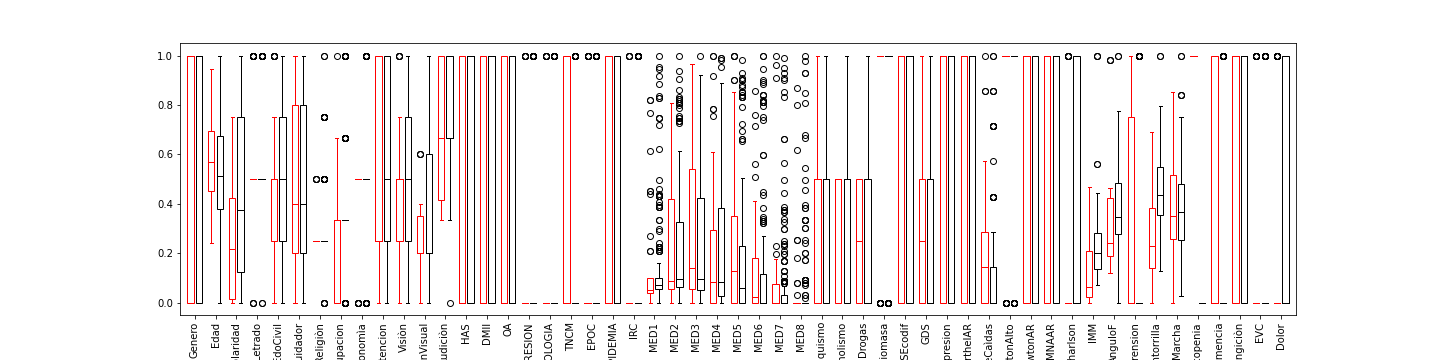
\includegraphics[width=\linewidth]{boxplot_serve_mild.png}
\caption{Boxplot of all remaining features, black boxes are from all mild cases and red from all serve, respectively}
\label{fig:boxplots}
\end{figure*} 
\end{document}
